
% Quantum Computation

\section{محاسبات کوانتومی}

\subsection{سیستم‌های تک‌کیوبیتی}

طبق قوانین فیزیک کوانتومی، حالت یک سیستم می‌تواند به صورت ترکیب خطی‌ای از چند حالت پایه باشد، که این حالت‌های پایه، حالت‌هایی هستند که در قوانین فیزیک کلاسیک نیز حالات صحیحی برای توصیف سیستم هستند.
در محاسبات کوانتومی از بردارهای عمودی برای نشان‌دادن وضعیت یک سیستم استفاده می‌شود و وضعیت سیستم‌های چندکیوبیتی را نیز می‌توان از روی بردارهای یک سیستم تک‌کیوبیتی نیز ساخت.
\\
به طور معمول، در محاسبات کوانتومی، صرفا سیستم‌هایی که دارای تنها دو حالت پایه هستند بررسی می‌شوند، به همین علت، بردارهای فضای حالات سیستم‌های تک‌کیوبیتی دو بعدی هستند. لذا دو بردار مستقل یکه به عنوان بردارهای پایه‌ی این فضا تعیین داده می‌شوند که رابطه‌ی یک به یک ای با حالات پایه‌ی بیت‌های کلاسیک دارند.
این حالات پایه به صورت زیر تعیین می‌شوند:
\begin{equation}
    |0\rangle = \begin{bmatrix} 1 \\ 0 \end{bmatrix} 
    \mspace{18mu}
    |1\rangle = \begin{bmatrix} 0 \\ 1 \end{bmatrix}
\end{equation} 
\myequations{بردارهای پایه تک‌کیوبیتی}

نشان دادن بردارهای حالت به صورت 
\lr{$|0\rangle$} و \lr{$|1\rangle$}
به نمادگذاری برا-کت دیراکت
\fnote{Dirac's bra-ket notation}
معروف است و به ازای هر کت
به صورت زیر:
\begin{equation}
    |\psi\rangle = \alpha |0\rangle + \beta |1\rangle
    = \begin{bmatrix}
    \alpha \\[3pt]
    \beta
    \end{bmatrix}
\end{equation}
یک برا
به این صورت تعریف می‌شود:
\begin{equation}
    \langle \psi| = \alpha^* \langle0| + \beta^* \langle1| = \begin{bmatrix} \alpha^* & \beta^* \end{bmatrix} 
\end{equation}

که در این‌جا نماد \lr{$\alpha^*$}
به معنای مزدوج مختلط 
\fnote{Complex conjugate}
عدد \lr{$\alpha$}
است.
\newpage

حالت‌های سیستم در فیزیک کوانتومی در اکثر اوقات به صورت بردارهای مختلط بهنجار
\fnote{Normalizable}
نشان داده می‌شوند.
\begin{equation}
    |\psi\rangle = \alpha |0\rangle + \beta |1\rangle = \begin{bmatrix} \alpha \\ \beta \end{bmatrix} 
    ; \mspace{18mu}
    \alpha, \beta \in \mathbb{C}
\end{equation}
% \newpage
\myequations{فرم کلی بردار وضعیت سیستم تک کیوبیتی}
که به امر ایجاد یک بردار وضعیت از ترکیب خطی دو بردار وضعیت دیگر، اصل برهم‌نهی کوانتومی
\fnote{Quantum Superposition}
گفته می‌شود.

بهنجار بودن به معنای صدق شرایط زیر است:
\begin{equation}
    \alpha\alpha^* + \beta\beta^* = |\alpha|^2 + |\beta|^2 = 1
\end{equation}
\myequations{شرط بهنجار بودن}
% \newpage
\begin{figure}
	\centering
	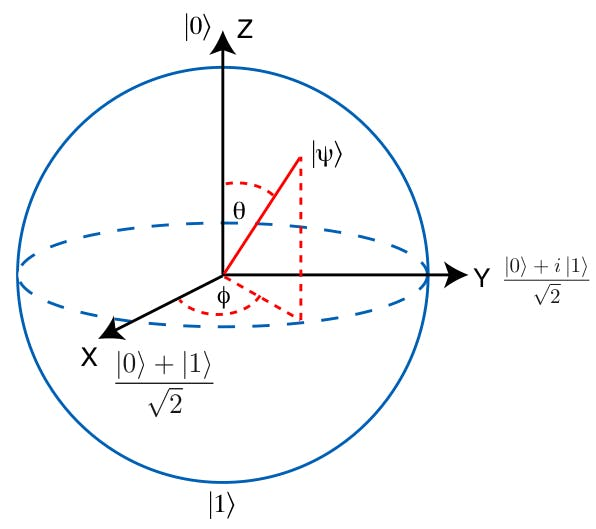
\includegraphics[scale=0.4]{figures/bloch.jpg}
	\caption{کره‌ی بلاخ}
	\label{fig:bloch}
\end{figure}
به علت شرط بهنجاری، می‌توان حالت کلی یک سیستم تک‌کیوبیتی را به صورت زیر نیز نوشت:
\begin{equation}
|\psi\rangle = \begin{bmatrix} e^{i\phi_1}\cos{\tfrac{\theta}{2}} \\[6pt] e^{i\phi_2}\sin{\tfrac{\theta}{2}} \end{bmatrix} 
\mspace{18mu}
\theta, \phi_1, \phi_2 \in {\rm I\!R}
\end{equation}
\myequations{حالت معادل فرم کلی بردار تک‌کیوبیتی}

که آن را می‌توان به صورت زیر نیز نوشت:
\begin{equation}
|\psi\rangle = e^{i\phi_1} \begin{bmatrix} \cos{\tfrac{\theta}{2}} \\[6pt] e^{i\phi_2-\phi_1}\sin{\tfrac{\theta}{2}} \end{bmatrix} = e^{i\phi_1} \begin{bmatrix} \cos{\tfrac{\theta}{2}} \\[6pt] e^{i\phi}\sin{\tfrac{\theta}{2}} \end{bmatrix}
\Rightarrow |\psi\rangle = \begin{bmatrix} \cos{\tfrac{\theta}{2}} \\[6pt] e^{i\phi}\sin{\tfrac{\theta}{2}} \end{bmatrix}
\end{equation}
\myequations{مهم نبودن فاز کلی سیستم}
در این معادله،
\lr{$\phi_1$}
 فاز کلی سیستم نامیده می‌شود که طبق قوانین فیزیک کوانتومی، در رفتار سیستم فاقد اهمیت است و به همین علت در مرحله‌ی آخر از آن صرف نظر شده است. \\
در نهایت، حالت کلی یک کیوبیت را می‌توان با استفاده از ابزاری به نام کره‌ی بلاخ (شکل
\ref{fig:bloch})
نمایش داد.

\subsection{سیستم‌های چندکیوبیتی}
دو سیستم تک‌کیوبیتی جداگانه را می‌توان به طور مجزا و به صورت زیر نمایش داد:
\begin{equation}
|a\rangle = \begin{bmatrix} a_0 \\ a_1 \end{bmatrix}, \quad |b\rangle = \begin{bmatrix} b_0 \\ b_1 \end{bmatrix}
\end{equation}
\myequations{دو کیوبیت مجزا}
در عین حال، می‌توانیم بردار وضعیت آن‌ها را به صورت هم‌زمان با استفاده از عملگری به نام ضرب تانسوری\fnote{Tensor product}
تعریف کنیم که به صورت زیر عمل می‌کند:
\begin{equation}
|b\rangle \otimes |a\rangle = \begin{bmatrix} b_0 \times \begin{bmatrix} a_0 \\ a_1 \end{bmatrix} \\[12pt] b_1 \times \begin{bmatrix} a_0 \\ a_1 \end{bmatrix} \end{bmatrix} = \begin{bmatrix} b_0 a_0 \\[2pt] b_0 a_1 \\[2pt] b_1 a_0 \\[2pt] b_1 a_1 \end{bmatrix} = |ba\rangle
\end{equation}
\myequations{ضرب تانسوری}

\subsection{درهم‌تنیدگی}

درهم‌تنیدگی کوانتومی\fnote{Quantum Entanglement}،
یکی از اصول فیزیک کوانتومی است و به این معناست که برخی بردار وضعیت‌های سیستم‌های چندکیوبیتی را نمی‌توان به صورت ضرب تانسوری دو بردار تک‌کیوبیتی مجزا تعریف کرد. این امر نشان‌گر این است که وضعیت این دو کیوبیت به هم وابسته هستند.
به عنوان مثال، اگر بردارهای زیر که در محاسبات کوانتومی به وضعیت‌های بل 
\fnote{Bell states}
معروف هستند در نظر گرفته شوند:
\begin{equation}
|{\Phi_\pm}\rangle = \frac{1}{\sqrt 2}\big(|0\rangle| 0\rangle\pm |1\rangle| 1\rangle\big), \qquad |{\Psi_{\pm}}\rangle=\frac{1}{\sqrt 2}\big(|0\rangle| 1\rangle\pm  |1\rangle|0\rangle\big)
\end{equation}
\myequations{بردار وضعیت‌های بل}
\hsm
مشاهده می‌شود که هیچ‌کدام از این بردارها را نمی‌توان به صورت ضرب تانسوری‌ای از ترکیب خطی بردارهای
\lr{$|0\rangle$} و \lr{$|1\rangle$}
نوشت.

\subsection{گیت‌های کوانتومی}
در کامپیوترهای کلاسیک، محاسبات با استفاده از گیت‌هایی همانند 
\lr{AND}، \lr{OR} و NOT
انجام می‌شود.
معادل این گیت‌ها در محاسبات کوانتومی، گیت‌های کوانتومی هستند. این گیت‌ها به فرم ماتریس‌های یکانی 
\fnote{Unitary matrix}
\lr{$2^n \times 2^n$}
هستند که در این‌جا، عدد \lr{$n$}
نشان‌گر تعداد کیوبیت‌های سیستم است.
به دلیل استفاده از گیت‌های کوانتومی، الگوریتم‌های کوانتومی به نام مدارهای کوانتومی نیز مطرح هستند و عمق یک مدار کوانتومی، به معنای بیشینه‌ی تعداد گیت‌هایی است که بر روی هر کدام از کیوبیت‌ها اعمال می‌شود.
\subsubsection{
    گیت‌های کوانتومی تک‌کیوبیتی
}
در این بخش، صرفا تعدادی از گیت‌های کوانتومی به صورت خلاصه معرفی می‌شوند و اثر آن‌ها بر روی پایه‌های برداری فضای سیستم‌های تک‌کیوبیتی نشان داده می‌شود؛ چراکه تاثیر این گیت‌ها بر بردار وضعیت کیوبیت‌های دل‌خواه، با استفاده از ترکیب خطی تاثیر این گیت‌ها بر پایه‌های برداری به دست می‌آید.
\begin{equation}
X = \begin{bmatrix} 0 & 1 \\ 1 & 0 \end{bmatrix} \qquad
Y = \begin{bmatrix} 0 & -i \\ i & 0 \end{bmatrix} \qquad
Z = \begin{bmatrix} 1 & 0 \\ 0 & -1 \end{bmatrix} \qquad
H = \frac{1}{\sqrt{2}} \begin{bmatrix} 1 & 1 \\ 1 & -1 \end{bmatrix}
\end{equation}
\myequations{گیت‌های پائولی و هادامارد}
گیت‌های 
$X, Y, Z$
به گیت‌های پائولی
\fnote{Pauli gates}
و گیت
$H$
به گیت هادامارد
\fnote{Hadamard gate}
معروف است.
تمامی گیت‌های تک‌کیوبیتی، حالت خاصی از گیت پارامتردار 
\lr{$U_3$}
هستند.

\begin{equation}
U_3(\theta, \phi, \lambda) = \begin{bmatrix} \cos(\frac{\theta}{2}) & -e^{i\lambda}\sin(\frac{\theta}{2}) \\[6pt]
            e^{i\phi}\sin(\frac{\theta}{2}) & e^{i(\phi+\lambda)}\cos(\frac{\theta}{2})
     \end{bmatrix}
\end{equation}
\myequations{گیت \lr{$U_3$}}

گیت‌های دوران پائولی
\fnote{Pauli rotation}
، گیت‌هایی هستند که با استفاده از رابطه‌های زیر به دست می‌آیند و به معنای چرخش وضعیت کیوبیت حول محورهای مختصات مختلف با زاویه‌ی 
$\phi$
هستند.
\begin{equation}
\begin{gathered}
    R_x(\phi) = e^{-i \phi X/2} = 
            \begin{bmatrix}
                \cos(\phi/2) & -i\sin(\phi/2) \\
                -i\sin(\phi/2) & \cos(\phi/2)
            \end{bmatrix}
            \\[3pt]
    R_y(\phi) = e^{-i\phi Y/2} = 
            \begin{bmatrix}
                \cos(\phi/2) & -\sin(\phi/2) \\
                \sin(\phi/2) & \cos(\phi/2)
            \end{bmatrix}
            \\[3pt]
    R_z(\phi) = e^{-i\phi Z/2} = \begin{bmatrix}
                e^{-i\phi/2} & 0 \\
                0 & e^{i\phi/2}
            \end{bmatrix}
\end{gathered}
\end{equation}
\myequations{گیت‌های دوران پائولی}

\subsubsection{
    گیت‌های کوانتومی چند‌کیوبیتی
}
گیت‌های چندکیوبیتی نیز، همانند بردارهای وضعیت سیستم‌های چندکیوبیتی، دو نوع متفاوت دارند. در این بخش -برای سادگی محاسبات- تنها گیت‌های دوکیوبیتی را بررسی می‌کنیم؛ اما همین روابط برای تعداد کیوبیت‌های بالاتر نیز صادق است. \\
نوع اول، گیت‌هایی هستند که می‌توان آن‌ها را به صورت ضرب تانسوری دو گیت تک‌کیوبیتی تجزیه کرد.
\\
به عنوان مثال:
\begin{equation}
    \begin{bmatrix}
    0 & 1 & 0 & 0 \\[3pt]
    1 & 0 & 0 & 0 \\[3pt]
    0 & 0 & 0 & 1 \\[3pt]
    0 & 0 & 1 & 0 
    \end{bmatrix} =
    \begin{bmatrix}
    1 & 0 \\[3pt]
    0 & 1 
    \end{bmatrix} \otimes
    \begin{bmatrix}
    0 & 1 \\[3pt]
    1 & 0
    \end{bmatrix}
    = \mathbb{I} \otimes X
\end{equation}
\myequations{گیت چندکیوبیتی ترکیبی}
این گیت معادل این است که هم‌زمان یک گیت همانی یا
$\mathbb{I}$
بر روی کیوبیت اول و یک گیت
$X$
بر روی کیوبیت دوم اعمال شود.

نوع دوم، گیت‌هایی هستند که به ضرب تانسوری دو گیت تک‌کیوبیتی تجزیه‌پذیر نیستند و تنها همین نوع گیت‌ها هستند که در هنگام اعمال بر روی برخی از حالت‌های کیوبیتی برهم‌نهاده، منجر به ایجاد درهم‌تنیدگی می‌شوند، به عنوان مثال، گیت
$CNOT$
\fnote{Controlled NOT}
به این صورت تعریف می‌شود:
\begin{equation}
    CNOT = \begin{bmatrix}
    1 & 0 & 0 & 0 \\[3pt]
    0 & 1 & 0 & 0 \\[3pt]
    0 & 0 & 0 & 1 \\[3pt]
    0 & 0 & 1 & 0 
    \end{bmatrix}
\end{equation}
\myequations{گیت CNOT}

به عنوان یک مثال از ایجاد درهم‌تنیدگی و برهم‌نهی، می‌توان دید:
\begin{equation}
    CNOT(H \otimes \bbmath{I}(|00\rangle)) = CNOT(\frac{1}{\sqrt{2}} \big( |0\rangle + |1\rangle \big) \otimes |0\rangle ) = \frac{1}{\sqrt{2}} (|00\rangle + |11\rangle)
\end{equation}
\myequations{تاثیر گیت \lr{CNOT} در ایجاد درهم‌تنیدگی}
این گیت به این دلیل نام‌گذاری شده که تاثیر آن بر روی کیوبیت دوم، توسط وضعیت کیوبیت اول کنترل شده؛ به این معنا که تنها در صورتی که کیوبیت اول در وضعیت
$|1\rangle$
باشد، گیت 
$X$
بر روی کیوبیت دوم اعمال خواهد شد.

\subsection{اندازه‌گیری}
اندازه‌گیری در محاسبات کوانتومی را می‌توان به گونه‌های مختلفی تعریف کرد، در این متن، یکی از این شیوه‌ها به عنوان معیار در نظر گرفته شده و تنها به آن پرداخته می‌شود.
عمل اندازه‌گیری در فیزیک کوانتومی، یک بردار وضعیت (که ممکن است برهم‌نهاده باشد) را به عنوان ورودی گرفته و یک عدد حقیقی بین
$0$
و
$1$
را به عنوان خروجی می‌دهد.
این اندازه‌گیری‌ها با توجه به یک مشاهده‌پذیر 
\fnote{Observable}
انجام می‌گیرند. مشاهده‌پذیرها در فیزیک کوانتومی، ماتریس‌های هرمیتی
\fnote{Hermitian matrix}
هستند. در این متن، فرض می‌شود که همیشه اندازه‌گیری با توجه به مشاهده‌پذیر 
$Z$
انجام می‌شود و به صورت زیر تعریف می‌شود:
\begin{equation}
    \langle \psi| Z^{\otimes n} | \psi\rangle
\end{equation}
\myequations{اندازه‌گیری کوانتومی}
\hsm
که
$n$
تعداد کیوبیت‌های سیستم است. به عنوان مثال:
\begin{equation}
    \langle 1 | Z | 1 \rangle = 
    \begin{bmatrix}
    0 & 1
    \end{bmatrix} 
    \begin{bmatrix}
    1 & 0 \\[3pt]
    0 & -1 \\[3pt]
    \end{bmatrix}
    \begin{bmatrix}
    0 \\[3pt] 1
    \end{bmatrix} 
    = \begin{bmatrix}
    0 & 1
    \end{bmatrix} 
    \begin{bmatrix}
    0 \\[3pt] -1
    \end{bmatrix}
    = -1
\end{equation}
\myequations{مثال اندازه‌گیری کوانتومی}
\hsm
که معادل قرار گرفتن وضعیت کیوبیت بعد از اندازه‌گیری در حالت 
$|1\rangle$
خواهد بود. در صورتی که بردار موردنظر دچار برهم‌نهی باشد،امیدریاضی اندازه‌گیری‌های متعدد به عنوان خروجی اندازه‌گیری در نظر گرفته می‌شود.

در صورتی که این اندازه‌گیری‌ها به صورت جداگانه بر روی کیوبیت‌های سیستم اعمال شوند و در سیستم در‌هم‌تنیدگی وجود داشته‌باشد؛ درایه‌های آرایه‌ای که از این اندازه‌گیری‌ها به وجود می‌آید به میزان درهم‌تنیدگی موجود در سیستم با هم مرتبط خواهند بود. به عنوان مثال، اگر در سیستم
$\frac{1}{\sqrt{2}} (|00\rangle + |11\rangle)$
کیوبیت اول اندازه‌گیری شود و بعد از اندازه‌گیری در حالت 
$|0\rangle$
قرار بگیرد، کیوبیت دوم نیز حتما در حالت
$|0\rangle$
خواهد بود و بالعکس.

\subsection{یادگیری ماشین کوانتومی}

یادگیری ماشین کوانتومی به مجموعه‌ای از الگوریتم‌ها اطلاق می‌شود که از ادغام الگوریتم‌های کوانتومی در مدل‌های یادگیری ماشین ایجاد شده‌اند. این الگوریتم‌ها به دو نوع هستند: در نوع اول، تمامی  قسمت‌های الگوریتم یادگیری ماشین فرم کوانتومی به خود می‌گیرند؛ و در نوع دوم، برخی از زیر روال‌ها
\fnote{Subroutine}
ی مدل یادگیری ماشین، با الگوریتم کوانتومی معادلی جای‌گزین می‌شوند. الگوریتم‌های نوع دوم، به الگوریتم‌های ترکیبی کوانتوم-کلاسیک معروف هستند و در حال حاضر که در عصر
کامپیوترهای کوانتومی نویزدار مقیاس متوسط
\fnote{Noisy intermediate-scale quantum (NISQ) computers}
قرار داریم، به طور معمول کاربرد بیش‌تری دارند، چراکه زیرروال‌های کوانتومی استفاده شده در این الگوریتم‌ها عمدتا به تعداد کیوبیت‌های کم‌تری لازم دارند و مدار کم‌عمق‌تری دارند. \\

الگوریتم‌های یادگیری ماشین کوانتومی به طور کلی از دو بخش کدگذاری
\fnote{Encoding}
و بخش پارامتریک
\fnote{Variational}
تشکیل شده‌اند.
بخش کدگذاری با دریافت یک داده به عنوان ورودی، با استفاده از روش‌های کگذاری داده‌ی کوانتومی
\fnote{Quantum data encoding}
وضعیت اولیه‌ی کیوبیت‌ها را به نسبت داده‌های ورودی تغییر می‌دهد.
بخش پارامتریک حاوی پارامترهای تغییرپذیر است که با توجه به الگوریتم گرادیان کاهشی، برای کمینه کردن تابع هزینه بهینه‌سازی می‌شود.

در یادگیری ماشین کوانتومی، می‌توان اثبات کرد که اگر یک مدار کوانتومی پارامتردار
$f(x; \theta)$
از گیت‌های دوران پائولی و 
$CNOT$
تشکیل شده باشد، گرادیان آن را می‌توان به صورت زیر نوشت
\cite{Mitarai}:
\begin{equation}
    \nabla f(x; \theta) 
    = \frac{1}{2} \hso [f(x;\theta + \frac{\pi}{2}) - f(x; \theta - \frac{\pi}{2})]
\end{equation}
\myequations{قانون انتقال پارامتر}
\hsm
که این رابطه به قانون انتقال پارامتر
\fnote{Parameter-shift rule}
معروف است.

\subsubsection{حافظه‌ی طولانی کوتاه مدت کوانتومی} \label{sec:qlstm}
الگوریتم حافظه‌ی طولانی کوتاه مدت کوانتومی، از جای‌گذاری گیت‌های بازگشتی الگوریتم حافظه‌ی طولانی کوتاه مدت با معادل کوانتومی آن‌ها ایجاد شده‌است، به این معنا که خروجی گیت‌های بازگشتی، برابر با امیدریاضی اندازه‌گیری کیوبیت‌های یک مدار کوانتومی پارامتردار هستند. 
ساختار درونی این مدارهای کوانتومی پارامتردار متغیر هستند و بسته به مساله‌ی مورد بررسی، می‌توانند صورت‌های مختلفی به خود بگیرند.

\subsubsection{شبکه‌های زایای دشمن‌گونه‌ی کوانتومی} \label{sec:qugan}
ساختار کلی شبکه‌های زایای دشمن‌گونه‌ی کوانتومی که در شکل 
\ref{fig:qugan}
آمده است، به طور معمول متشکل از سه زیرروال کوانتومی به صورت زیر است:

زیرروال اول همان مدار کدگذاری است که با گرفتن داده‌ی ورودی، آن را در وضعیت کیوبیت‌ها کدگذاری می‌کند.

زیرروال دوم، زیرروال تشخیص است که با دریافت داده‌ی کدگذاری شده در وضعیت کیوبیت‌ها، سعی می‌کند تشخیص دهد که داده‌ی فعلی، یک داده‌ی واقعی از مجموعه داده‌ها است یا یک داده‌ی ساختگی که از جای دیگری تولید شده‌است.

زیرروال سوم، زیرروال زایا است که با دریافت یک ورودی تصادفی به عنوان نویز، سعی می‌کند داده‌ی جدیدی که شبیه به داده‌های مجموعه داده باشد تولید کند. گرفتن نویز به این علت است که زیرروال زایا همیشه یک خروجی ثابت تولید نکند و خروجی آن در هر بار خروجی‌ای بدیع و نوین باشد.

به خاطر ساختار ذاتی مدارهای کوانتومی، شبکه‌های زایای دشمن‌گونه‌ی کوانتومی متشکل از دو مدار هستند.
مدار داده‌ی واقعی، ابتدا با استفاده از زیرروال کدگذاری، داده‌های واقعی را در وضعیت کیوبیت‌ها کدگذاری می‌کند؛ سپس با استفاده از زیرروال تشخیص، سعی می‌کند ساختار داده‌های واقعی را یاد بگیرد.

مدار داده‌ی ساختگی، ابتدا با استفاده از زیرروال کدگذاری، یک نویز را به عنوان ورودی می‌گیرد و این نویز را  در وضعیت کیوبیت‌ها کدگذاری می‌کند؛ سپس با استفاده از زیرروال زایا، سعی می‌کند داده‌های جدیدی تولید کند و در نهایت با استفاده از زیرروال تشخیص، سعی می‌کند ساختگی یا واقعی بودن داده را تشخیص دهد.

نکته‌ی مهم این است که زیرروال‌های تشخیص استفاده شده در این دو مدار، پارامترهای یکسانی دارند، به این معنا که حتی بعد از آپدیت‌شدن این پارامترها در یک مدار، پارامترهای مدار دیگر نیز تغییر خواهند کرد.

تابع هزینه‌های زیرروال تشخیص که با 
$D$
و زیرروال زایا که با
$G$
نشان داده می‌شود، به صورت زیر تعریف می‌شود:
\begin{equation} \label{eqn:qugan_cost}
    \begin{gathered}
        Cost_D = Pr(real|fake) - Pr(real|real)  \\
        Cost_G = -Pr(real|fake)
    \end{gathered}
\end{equation}
\myequations{توابع هزینه‌ی شبکه‌ی زایای دشمن‌گونه‌ی کوانتومی}
به این معنا که زیرروال تشخیص تلاش می‌کند احتمال تشخیص داده‌ی واقعی به عنوان داده‌ی واقعی را افزایش دهد، در حالی که احتمال تشخیص داده‌ی ساختگی به عنوان داده‌ی واقعی را کم کند؛ در حالی که زیرروال زایا تلاش می‌کند تا احتمال تشخیص خروجی تولید شده‌اش توسط زیرروال تشخیص به عنوان داده‌ی واقعی را افزایش دهد.


\begin{figure}
	\centering
	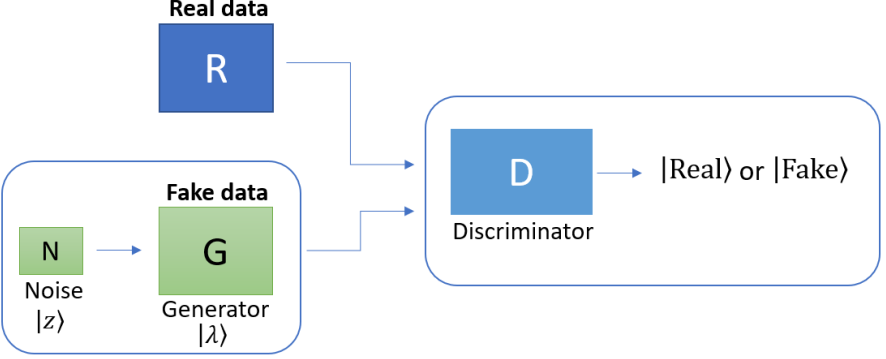
\includegraphics[scale=0.4]{figures/qugan.png}
	\caption{شبکه‌ی زایای دشمن‌گونه‌ی کوانتومی}
	\label{fig:qugan}
\end{figure}



